\documentclass{standalone}
\usepackage{tikz}
\usepackage{animate}
\usepackage{amsmath}
\usepackage{ifthen}
\usetikzlibrary {matrix}
\usepackage{tikzlings}
\usepackage{tikzlings-penguins}

\begin{document}
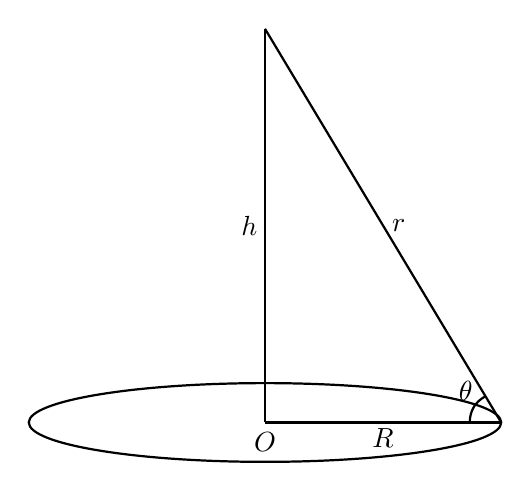
\begin{tikzpicture}[>=latex,thick]
  \begin{scope}
    \coordinate  (O) at (0,0) node[below] {$O$}; 
    \coordinate   (a) at (3,0) ;
    \coordinate  (b) at (0,5) ;
    \draw  (O)--(a);
    \node  (r) at (1.7,2.5) {$r$};
    \draw (O) --(b) ;
    \node (h) at (-0.2,2.5) {$h$};
    \draw (a)--(b)  ;
    \node (R) at (1.5,-0.2) {$R$};
    \draw (0,0) circle [x radius=3, y radius=0.5];
    \draw[bend left] (2.6,0) to (2.8,0.3335); 
    \node (theta) at (2.55,0.4) {$\theta$};
  \end{scope}

\end{tikzpicture}


\end{document}
